% geometrische simplizialkomplexe

\section{Geometrische Simplizialkomplexe}

Die geometrischen Simpliziale alleine reichen nicht aus, um einen
komplizierten topolgischen Raum zu beschreiben bzw. modellieren. Denn
ein $\sigma^n$ ist nach \cref{satz:simp} isomorph zu $\Bn$.  Mithilfe
von Komplexen von Simplizialen können nun kompliziertere topologische
Räume modelliert werden.

\begin{Def}[Geometrischer Simplizialkomplex]
  Wir nennen eine nicht leere Menge $\Delta$ von (geometrischen) Simplizialen
  einen \textbf{geometrischen Simplizialkomplex} oder einfach
  geometrischer Komplex, falls er folgende Bedingungen $(K1) - (K3)$
  erfüllt.
  \begin{enumerate}[(K1)]
  \item $\emptyset \in \Delta$
  \item Für jeden Simplex $\sigma \in \Delta$ ist auch jede Seite
    $\tau$ von $\sigma$ in $\Delta$ enthalten.
  \item Mit allen Simplexen $\sigma, \sigma' \in \Delta$ ist auch ihr
    Schnitt $\sigma \cap \sigma'$ in $\Delta$ enhalten.
  \item[(K4)] Für zwei verschiedene Simplexe $\sigma,\tau \in \Delta$
    gilt $\Int(\sigma) \cap \Int(\tau) = \emptyset$.
  \end{enumerate}
\end{Def}


\begin{Bsp}
  \begin{enumerate}[(1)]
  \item Sei $\sigma^n \coloneqq e_0 \ldots e_n $ der Standardsimplex.
    Die Menge aller Seiten von $\sigma^n$ bildet einen geometrischen
    Simplizialkomplex.
  \item Hier ist ein Standardbeispiel eines Komplexes abgebildet\\
    \begin{center}
    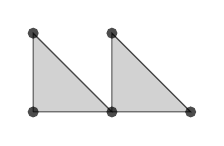
\begin{tikzpicture}[opacity=0.7]
        \draw [thin,fill=lightgray] (0,0) to (1,0) to (0,1) to (0,0);
        \draw [thin,fill=lightgray] (1,0) to (2,0) to (1,1) to (1,0);
        \fill (0,0) circle[radius=0.07cm];
        \fill (1,0) circle[radius=0.07cm];
        \fill (0,1) circle[radius=0.07cm];
        \fill (2,0) circle[radius=0.07cm];
        \fill (1,1) circle[radius=0.07cm];
    \end{tikzpicture}
  \end{center}
  und eine Menge von Simplizialen die keinen Komplex bilden.
  \begin{center}
  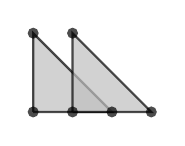
\begin{tikzpicture}[opacity=0.7]
        \draw [thick,fill=lightgray] (0,0) to (1,0) to (0,1) to (0,0);
        \draw [thick,fill=lightgray] (0.5,0) to (1.5,0) to (0.5,1) to (0.5,0);
        \foreach \foo in {(0,0),(1,0),(0,1),(0.5,0),(1.5,0),(0.5,1)}
        \fill \foo circle[radius=0.07cm];
    \end{tikzpicture}
  \end{center}
\item Ein Komplex muss weder endlich noch beschränkt sein.\\
    \begin{tikzpicture}
      \draw [ultra thin] (-0.5,0) to (10.5,0); 
      \node (r) at (11,0) {$= \R$};
      \draw (-0.5,-1)--++(11,0);
      \foreach \foo in {0,...,10}
      \fill (\foo,-1) circle[radius=0.07cm];
    \end{tikzpicture}

    Der zweite Komplex füllt die reelle Achse vollkommen aus. Dieses Ausfüllen
    wird nun durch folgende Definition näher erläutert.

\end{enumerate}
\end{Bsp}

\begin{Def}[Unterkomplex, $k$-Skelett, Dimension, Polyeder]
  Sei $\Delta$ ein geometrischer Komplex, so definiere
  \begin{enumerate}[(a)]
  \item Eine Teilmenge $\Delta'$ von $\Delta$ heißt
    \textbf{Unterkomplex}, falls $\Delta'$ wiederum einen
    Simplizialkomplex bildet.
  \item Die Dimension eines Simplizialkomplexes ist wie folgt
    definiert:
    \begin{gather*}
      \dim(\Delta) \coloneqq \sup \left\{ \dim(\sigma) \; \Big| \;
        \sigma \in \Delta \right\}
    \end{gather*}
    Falls die Dimension unbeschränkt ist, wird diese auf unendlich
    gesetzt.
  \item Das \textbf{$k$-Skelett} $\Delta^{(k)}$ ist der Unterkomplex
    aller Simplizes mit der Dimension kleiner gleich $k$. Der
    Spezialfall $\Delta^{(0)}$ bezeichnet die \textbf{Eckmenge} von
    $\Delta$.
  \item Der \textbf{Polyeder} von $\Delta$ ist wie folgt definiert
    \begin{gather*}
      |\Delta| \coloneqq \bigcup \left\{ \sigma \; \Big| \; \sigma \in
        \Delta \right\} \subset \R^{\dim(\Delta)}.
    \end{gather*}
%    Der Polyeder entspricht dem Komplex dessen zugrundeliegender Raum.
    Dies entspricht dem Komplex zugrundeliegenden Raum.
  \item Eine Teilmenge von $\R^N$ heißt \textbf{triangulierbar}, falls
    sie homöomorph zu einem Polyeder eines geometrischen Komplexes
    sind.
  \end{enumerate}
\end{Def}

Zur Veranschaulichung der vorher definierten Begriffe ein Beispiel.

\begin{Bsp}\label{bsp:triangulierung}
  \begin{description}
  \item[Skelette:] Betrachte den folgenden Komplex $\Delta$ mit $\dim(\Delta)=2$\\
    \begin{center}
    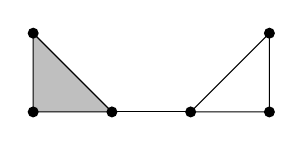
\begin{tikzpicture}
      \draw [thin,fill=lightgray] (0,0) to (1,0) to (0,1) to (0,0);
      \draw [thin] (1,0) to (2,0);
      \draw [thin] (2,0) to (3,0) to (3,1) to (2,0);
      \foreach \foo in {(0,0),(1,0),(0,1),(2,0),(3,0),(3,1)}
      \fill \foo circle[radius=0.07cm];      
    \end{tikzpicture}
  \end{center}
  Dann gibt es zu diesem Komplex folgende $k$-Skelette\\
  \begin{center}
    \parbox{0.7\linewidth}{%
  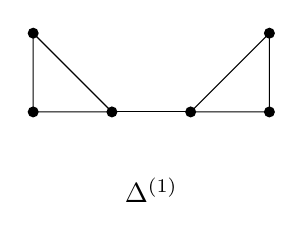
\begin{tikzpicture}
    \draw [thin] (0,0) to (1,0) to (0,1) to (0,0);
      \draw [thin] (1,0) to (2,0);
      \draw [thin] (2,0) to (3,0) to (3,1) to (2,0);
      \foreach \foo in {(0,0),(1,0),(0,1),(2,0),(3,0),(3,1)}
      \fill \foo circle[radius=0.07cm];      
      \node (a) at (1.5,-1) {$\Delta^{(1)}$};
  \end{tikzpicture}
  \hfill
  \begin{tikzpicture}
      \foreach \foo in {(0,0),(1,0),(0,1),(2,0),(3,0),(3,1)}
      \fill \foo circle[radius=0.07cm];      
      \node (a) at (1.5,-1) {$\Delta^{(0)}$};
  \end{tikzpicture}}
\end{center}  

\item[Triangulierung:] Betrachte den folgenden geometrischen Komplex
  $\Delta \coloneqq (\Delta^2)^{(1)}$. Also besitzt der Komplex von
  einem Dreieck die Seiten und Ecken. Das Polyeder von $\Delta$ ist
  homöomorph zur $\Sp^1$. Betrachte hierzu die stetige
  Normierungsabbildungabbildung
  $f : \R^2 \setminus \sset{0} \rightarrow \Sp^1 , x \mapsto
  \frac{x}{\nn[x]}$.
  Eingeschränkt auf den Polyeder von $\sigma$ erhält man eine stetige
  bijektive Abbildung und da die beiden Räume hausdorffsch und kompakt
  sind, muss die eingeschränkte Abbildung schon ein Homöomorphismus
  sein.
  \begin{center}
  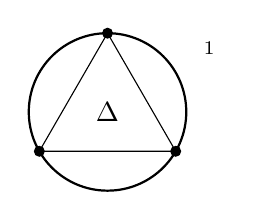
\begin{tikzpicture}
    \draw [thin] (90:1) to (210:1) to (330:1) to (90:1);
    \draw [thick] (0,0)circle(1cm);
    \foreach \foo in {90,210,330}
    \fill (\foo:1) circle[radius=0.07cm];

    \node (a) at (0,0) {$\Delta$};
    \node (b) at (30:1.5) {$\Sp^1$};
  \end{tikzpicture}
\end{center}
Anschaulich biegt man die Seiten nach außen auf den Kreisbogen. Somit
ist die $\Sp^1$ triangulierbar.
\end{description}
\end{Bsp}

\begin{Lem}\label{lem:eindeutigSimplex}
  Es gilt für eine Menge $\Delta$ folgende Äquivalenz
  \begin{enumerate}[(i)]
  \item (K1),(K2) und (K3)
  \item (K1),(K2) und (K4)
  \end{enumerate}
  Für eine Menge, die eine der obigen äquivalenten Aussagen erfüllt,
  gilt, dass für jeden Punkt $x \in \gr{\Delta}$ es genau ein
  $\sigma \in \Delta$ gibt, sodass $x \in \Int(\sigma)$ gilt.
  \begin{proof}
    \begin{description}
    \item[i) $\Rightarrow$ ii)] Sei zunächst $(K3)$ gegeben. Dann
      betrachte zu zwei verschiedenen Simplizialen
      $\sigma,\tau \in \Delta$ ihren Schnitt. Dieser ist nach
      Vorraussetzung wieder ein Simplex aus $\Delta$. Setze
      $s \coloneqq \sigma \cap \tau$ und zeige, dass falls
      $\Int(\sigma) \cap \Int(\tau)$ nicht leer ist die beiden
      Simpliziale übereinstimmen müssen. Sei
      $x \in \Int(\sigma) \cap \Int(\tau) \subset s$. Nun gilt, dass
      $s$ eine echte Seite von $\sigma$ oder $\tau$ sein muss. Es muss
      also gelten $s \subset \partial\sigma , \partial\tau$. Nach der
      vorherigen Wahl von $x$ aus den Inneren, kann dieser Punkt nun
      nicht im Rand liegen, also muss
      $\Int(\sigma) \cap \Int(\tau) = \emptyset$ gelten.
      \item[ii) $\Rightarrow$ i)] Übung.
    \end{description}
    Sei nun $\Delta$ ein geometrischer Komplex und
    $x \in \gr{\Delta}$, dann existiert offentsichlich ein Simplex
    $\sigma$ aus $\Delta$, sodass der Punkt aus diesem Simplex
    ist. Es kann nun aber auch stets das Innere von einem Simplex aus
    dem Komplex gewählt werden, denn falls für einen gewählten Simplex
    $\sigma$ der Punkt am Rand liegt, muss der Punkt nun auch in einer
    echten Seite enthalten sein. Für einen endlichen Komplex kann man
    nun stets einen Simplex finden, sodass der Punkt im Innneren
    liegt, sonst steige zu einer echten Seite ab.
  \end{proof}
\end{Lem}


Definiere auf dem zugrunde liegenden Raum eines Simplizialkomplexes eine 
Topologie.

\begin{Def}[schwache Topologie]
	Sei $\Delta$ ein Simplizalkomplex, dann definiere die
	\textbf{schwache Topologie} auf dem Polyeder $\gr{\Delta}$
	durch folgende Charakterisierung der abgeschlossenen Mengen.
	\begin{gather*}
          A \subset \gr{\Delta} \text{ abgeschlossen }
          :\Leftrightarrow A \cap \sigma \text{ abgeschlossen für alle
          } \sigma \in \Delta
	\end{gather*}
	Wobei auf der rechten Seite die Menge abgeschlossen bezüglich der
	Standardtopologie auf dem $\R^{\dim(\Delta)}$ ist.
\end{Def}

\begin{Lem}
  Die schwache Topologie ist feiner als die Standardtopologie und
  falls ein geometrischer Komplex $\Delta$ endlich ist, stimmen
  Standardtopologie und schwache Topologie auf $\gr{\Delta}$ überein.
  \begin{proof}
    Sei \OE\; $\gr{\Delta} \subset \R^N$ und $A \subset \gr{\Delta}$
    eine abgeschlossene Menge, so existiert ein $B \subset \R^N$
    abgeschlossen, sodass $A = B \cap \gr{\Delta}$ gilt. Nun gilt für
    jeden Simplex $\sigma \in \Delta$ folgende Gleichheit:
    $A \cap \sigma = B \cap \gr{\Delta} \cap \sigma = B \cap \sigma$
    und somit ist $A \cap \sigma$ abgeschlossen bezüglich $\sigma$,
    also abgeschlossen bezüglich der schwachen Topologie.
		
    Falls nun $\Delta$ eine endliche Menge von Simplizes ist, gilt für
    eine abgeschlossene Menge $A$ bezüglich $\gr{\Delta}$, dass
    $A \cap \sigma$ abgeschlossen in $\sigma$ ist und durch
    Vereinigung über die endlichen vielen Simplizes die
    Abgeschlossenheit bezüglich der Standardtopologie erreicht wird.
  \end{proof}
\end{Lem}

\begin{Bem}
  Die schwache Topologie ist im allgemeinen echt feiner als die
  Spurtopologie auf $\gr{\Delta}$ bezüglich dem $\R^N$. Betrachte
  hierzu den folgenden Simplizialkomplex,
  $\Delta \coloneqq \set{ \{t\} }{t \in \R}$.  Hierbei ist das Polyeder
  gleich zu $\R$, aber die schwache Topologie entspricht der
  Diskreten. Für eine beliebige Teilmenge von $A \subset \R$ ist der
  Schnitt $A \cap \{ t \}$ mit einen beliebigen $0$-Simplex aus
  $\Delta$ gleich dem Simplex selbst oder die leere Menge, somit stets
  abgeschlossen, also ist jede Teilmenge abgeschlossen und damit die
  schwache Topologie auf dem Polyeder der Diskreten und damit ungleich
  der Standardtopologie auf $\R$.
\end{Bem}

Auf dem Polyeder ist nun stets die schwache Topologie von der die Rede
ist, ausser es wird explizit die Spurtopologie von einem $\R^N$
verwendet.

Beweise nun einige Aussagen über die schwache Topologie.

\begin{Satz}
  Sei $\Delta$ ein Simplizialkomplex, so gelten folgende Aussagen
  \begin{enumerate}[(a)]
        \item Die schwache Topologie ist hausdorffsch.
        \item Sei $A \subset \gr{\Delta}$ eine kompakte Teilmenge,
          dann existiert ein endlicher Unterkomplex $\Delta'$ in
          dessen Polyeder $A$ enthalten ist. Insbesondere ist ein
          endlicher Komplex kompakt.
        \item Eine Abbildung $f: \gr{\Delta} \rightarrow X$ ist
          stetig, genau dann wenn $f_{| \sigma}$ für alle
          $\sigma \in \Delta$ stetig ist.
	\end{enumerate}
	\begin{proof}
          \begin{enumerate}[(a)]
          \item Sei $v \in \Delta^{(0)}$ ein Knoten, so definiere
            folgende Abbildungsvorschrift.  Nach
            \cref{lem:eindeutigSimplex} existiert für jeden Punkt $x$
            genau ein Simplex $\sigma \in \Delta$ mit
            $x \in \Int(\sigma)$. Falls nun $x$ in einem von $v$
            aufgespannten Simplex liegt, ist $t_v = t_i$ mit der
            baryzentrischen Darstellung $x = \sum^{n}_{i=0} t_i a_i$
            für $v=a_i $ und sonst $t_v = 0$.  Die Abbildung $t_v$ ist
            nun stetig, da die baryzentrischen Koordinaten stetig
            sind. Für zwei verschiedene Punkte
            $x_0,x_1 \in \gr{\Delta}$ existiert ein $r \in \R$ mit
            $t_v(x_0) < r < t_v(x_1)$, denn sonst würde durch die
            Eindeutigkeit der baryzentrischen Darstellung und der
            Verschiedenheit der Punkte ein Widerspruch folgen. So
            defniere folgende offene, disjunkte Umgebungen
            $U_1 \coloneqq \set{x}{ t_v(x)<r}$ und
            $U_2 \coloneqq \set{x}{ t_v(x)>r}$, so sind für je zwei
            Punkte disjunkte, offene Umgebungen konstruiert und der
            Raum ist hausdorffsch.
          \item Sei $A$ eine kompakte Teilmenge des Polyeders
            $\gr{\Delta}$, die in keinem endlichen Unterkomplex von
            $\Delta$ enthalten ist, so wähle je einen Punkt
            $x_\sigma \in A \cap \Int(\sigma)$, für alle $\sigma$ mit
            nichtleeren Schnitt mit $A$. Die Menge
            $\Sigma \subset \gr{\Delta}$ all dieser Punkte ist nicht
            endlich und besitzt als induzierte Topologie die
            Diskrete. Denn eine Teilmenge von $\Sigma$ hat stets
            endlichen Schnitt mit allen $\sigma \in \Delta$ und ist in
            der schwachen Topologie stets abgeschlossen, also sind
            alle Teilmengen abgeschlossen und die Menge $\Sigma$ somit
            diskret.
% TODO: suche quelle, nicht grundkurs-topologie
            Es ergibt sich nun ein Widerspruch dadurch, dass eine
            kompakte und nicht endliche Menge stets einen
            Häufungspunkt besitzt, die diskrete Menge $\Sigma$ aber
            keinen Häufungspunkt besitzten kann.
% TODO: eine diskrete, unendliche menge menge besitzt keinen häufungspunkt
            Somit muss die Menge $A$ in einem endlichen Unterkomplex
            enthalten sein. Es folgt nun unmittelbar, dass ein endlicher
            Komplex als endliche Vereinigung der kompakten Komplexe
            wiederrum kompakt ist.
          \item 
            \begin{description}
              % TODO: zeige noch für kohärente topologien, das bei der
              % definition abgeschlossen durch offen ersetzt werden
              % kann.
            \item[\glqq $\Rightarrow$\grqq] Falls die Abbildung
              bezüglich $\gr{\Delta}$ stetig ist, dann auch die
              Restriktion nach einem Unterraum
              $\sigma \subset \gr{\Delta}$.
            \item[\glqq $\Leftarrow$ \grqq] Sei $U \subset X$ offen,
              dann ist $f^{-1}(U) \cap \sigma$ für alle
              $\sigma \in \Delta$ nach Vorraussetzung wieder offen.
              Dann gilt aber
              \begin{align*}
                f^{-1}(U) &= f^{-1} (U) \cap \gr{\Delta} \\ 
                          &= f^{-1} (U) \cap \bigcup \set{\sigma }%
                            { \sigma \in \Delta} \\ 
                          &= \bigcup \set{ f^{-1}(U) \cap \sigma }%
                            { \sigma \in \Delta}
              \end{align*}
              ist als Vereinigung offener Mengen wieder offen.
            \end{description}
          \end{enumerate}
	\end{proof}
\end{Satz}

Definiere nun für spätere Zwecke Abbildungen zwischen Simplizialkomplexen.

\begin{Def}[Simpliziale Abbildung] 
  Seien zwei Simplizialkomplexe $\Delta, \Delta'$ gegeben, dann heißt
  eine Abbildung $f: \Delta^{(0)} \rightarrow \Delta'^{(0)}$ zwischen
  den Eckmengen eine \textbf{Simpliziale Abbildung}, falls für jeden
  Simplex $a_0 \ldots a_n$ aus $\Delta$ die Ecken auf einen Simplex
  $f(a_0) \ldots f(a_n)$ aus $\Delta'$ abgebildet werden. Man schreibt
  dann $f: \Delta \rightarrow \Delta'$.
\end{Def}

\begin{Satz} \label{satz:geosimp}
  Seien $\Delta, \Delta'$ zwei Simplizialkomplexe und
  $f: \Delta \rightarrow \Delta'$ eine simpliziale Abbildung, dann
  gelten folgende Aussagen
	\begin{enumerate}[(a)]
        \item $f(\Delta)$ ist ein Unterkomplex und das Urbild eines
          Unterkomplexes ist wieder ein Unterkomplex.
        \item Es gibt eine stetige Abbildung
          $\gr{f} : \gr{\Delta} \rightarrow \gr{\Delta'}$ die durch
          $f$ induziert wird und folgende Bedingung erfüllt:
          \begin{gather*}
            x = \sp{0}{n} t_i a_i \Rightarrow \gr{f}(x) = \sp{0}{n}
            t_i f(a_i)
          \end{gather*}
          Man nennt $\gr{f}$ die induzierte simpliziale Abbildung von
          $f$.
        \item Die Verkettung von induzierten simplizialen Abbildung
          ist wieder eine induzierte simpliziale Abbildung.
        \item Falls $f$ eine bijektive simpliziale Abbildung ist,
          deren Umkehrfunktion wiederrum simplizial ist, dann ist die
          induzierte Abbildung $\gr{f}$ ein Homöomorphismus. Wir
          nennen dann $\gr{f}$ oder auch $f$ einen simplizialen
          Homöomorphismus, bzw. Isomorphismus.
        \item Sei $\Delta$ ein endlicher simplizialer Komplex, dann
          existiert eine natürliche Zahl $N$, sodass $\Delta$
          isomorph zu einem Unterkomplex von $\Delta^N$ ist.
	\end{enumerate}
	\begin{proof}
          \begin{enumerate}[(a)]
          \item Prüfe die Axiome $(K1)-(K3)$ nach. $(K1)$ ist klar als
            Bild der leeren Menge. Sei $\sigma \in f(\Delta)$, dann
            existiert $\sset{a_i} \subset \Delta^{(0)}$, sodass
            $\sigma = f(a_0)\ldots f(a_n)$. Nun wird jede Seite von
            $\sigma$ durch eine Teilmenge von $\sset{a_i}$ aufgespannt
            und ist nun aufgrund der Eigenschaft der simplizialen
            Abbildung wiederrum aus $f(\Delta)$. 

            Für das Urbild eines Unterkomplexes ist nur zu $(K4)$ zu
            zeigen.  Dies folgt aber unmittelbar daraus, dass der
            Urbildoperator $f^{-1}$ mit $\Int$, Vereinigungen und
            Schnitten von Mengen vertauscht.
          \item Die Eindeutigkeit solch einer Abbildung ist klar, da
            sie linear auf den Punkten $a_i$ und $f(a_i)$ vorgegeben
            ist. 

            Die Abbildung ist zudem wohldefiniert, da die
            Koeffizienten von $\gr{f}(x)$ wieder in $[0,1]$ liegen und
            als Summe die $1$ ergeben. Zudem liegt der Punkt
            $\gr{f}(x)$ in $\gr{\Delta'}$, denn die simpliziale
            Abbildung $f$ bildet Simplexe auf Simplexe ab. Die
            Stetigkeit folgt unmittelbar daraus, dass die Abbildung
            stetig ist, als Abbildung von dem Simplex $a_0 \ldots a_n$
            nach $f(a_0)\ldots f(a_n)$ und nach der Definition der
            schwachen Topologie also auch als Abbildung bezüglich der
            Polyeder.
          \item Betrachte die Abbildungen
            $f : \Delta \rightarrow \Delta' , g : \Delta' \rightarrow
            \Delta''$.
            Dann ist die Verkettung $\gr{g} \circ \gr{f}$ für den Punkt
            $x = \sp{0}{n} t_i a_i \in \gr{\Delta}$
            \begin{gather*}
              \left( \gr{g} \circ \gr{f} \right) (x) = \gr{g} \left(
                \sp{0}{n} t_i f(a_i) \right) = \sp{0}{n} t_i g(f(a_i)
            \end{gather*}
            wieder eine simpliziale Abbildung, diese wird von
            $g \circ f$ induziert.
          \item Die induzierten Abbildungen $\gr{f},\gr{f^{-1}}$ sind
            stetig nach $(b)$. Es ist nur zu zeigen, dass diese
            zueinander inverse Abbildungen sind. Dies sieht man sofort
            aufgrund der Linearität ein bzw. für einen Punkt
            $x = \sp{0}{n} t_i a_i \in \gr{\Delta}$ folgt
            \begin{gather*}
              \left( \gr{f^{-1}} \circ \gr{f} \right) (x) =
              \gr{f^{-1}} \left( \sp{0}{n} t_i f(a_i) \right) =
              \sp{0}{n} t_i f^{-1}(f(a_i) = x
            \end{gather*}
            Ebenso die andere Richtung.
          \item Da der Komplex $\Delta$ endlich ist, besteht die
            Eckmenge $\Delta^{(0)} = \sset{ a_0 , \ldots a_n}$ aus
            $n+1$ unterschiedlichen Punkten, die nicht geometrisch
            unabhängig sein müssen. Sei nun zudem der Standardkomplex
            $\Delta^n$ mit $n+1$ geometrisch unabhängigen Punkten
            $\sset{b_0 \ldots , b_n}$ als Eckmenge dieses Komplexes
            gegeben.

            Betrachte nun zu den gegeben Daten die folgende
            simpliziale Abbildung
            $f : \Delta \rightarrow \Delta^n , a_i \mapsto b_i$.  Die
            Abbildung $f$ ist nach Konstruktion injektiv (also
            bijektiv, wegen den endlichen Mengen) und simplizial,
            falls man nun den Bildbereich noch auf den Komplex
            $f(\Delta)$ einschränkt, wird die Umkehrabbildung
            simplizial und nach $(d)$ ein Isomorphismus.
          \end{enumerate}
	\end{proof}
\end{Satz}

\begin{Bem}
  Nach \cref{satz:geosimp} $e)$ ist $\Delta^n$ das essentielle
  Beispiel für geometrische Komplexe, denn jeder endliche Komplex ist
  als ein isomorpher Unterkomplex in $\Delta^n$ enthalten.
\end{Bem}














%%% Local Variables:
%%% mode: latex
%%% TeX-master: "main"
%%% End: